\documentclass{slides}
\usepackage{./NTUEEbeamer}

\title[below title]{\textbf{Neural Tangent Kernel: On Double Descent}}
\author{Wen Perng (B10901042)}
\institute[NTU]{Physical Theories of (Machine) Learning}
\date{2025 Nov. 12}


\begin{document}

\maketitleframe


\begin{frame}{Overview: Double Descent}
    The generalization error can be separated into bias and variance:
    \begin{align*}
        \mathcal{E}_{g} &= \mathbb{E}_{\vec{x},\mathcal{D}}\left[\left(f_\star(\vec{x}) - f_{\vec{\theta}}(\vec{x})\right)^2\right] \\
        &= \mathbb{E}_{\vec{x}}\left[\left(\eqhl{teal}{\mathrm{Bias}(f_{\vec{\theta}},\vec{x})}\right)^2 + \eqhl{red}{\mathrm{Var}\left(f_{\vec{\theta}}(\vec{x})\right)}\right] \\
        &= \mathbb{E}_{\vec{x}}\left[\left(\eqhl{teal}{f_{\star}(\vec{x}) - \mathbb{E}_{\mathcal{D}}\left[f_{\vec{\theta}}(\vec{x})\right]}\right)^2 + \eqhl{red}{\mathbb{E}_{\mathcal{D}}\left[\left(f_{\vec{\theta}}(\vec{x}) - \mathbb{E}_{\mathcal{D}}\left[f_{\vec{\theta}}(\vec{x})\right]\right)^2\right]}\right]
    \end{align*}

    \vspace{-0.7cm}
    
    \begin{figure}
        \centering
        % \begin{tikzpicture}
        %     \draw[->] (0, 0) -- (6, 0) node[right] {$x$};
        %     \draw[->] (0, 0) -- (0, 3) node[above] {$y$};
        %     \draw[scale=0.5, domain=-3:3, smooth, variable=\x, blue] plot ({\x}, {\x*\x});
        %     \draw[scale=0.5, domain=-3:3, smooth, variable=\y, red]  plot ({\y*\y}, {\y});
        % \end{tikzpicture}
        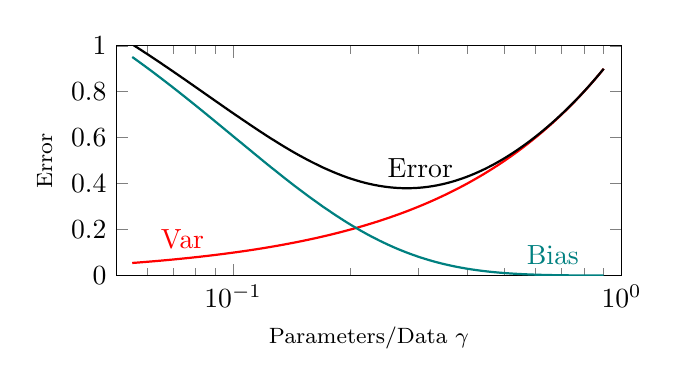
\begin{tikzpicture}
        \begin{axis}[
            width = 8cm, height = 4.5cm,
            xmax = 1, xmin = 0.05, xmode = log, xlabel = {\footnotesize Parameters/Data $\gamma$},
            ymax = 1, ymin = 0, ymode = normal, ylabel = {\footnotesize Error}
        ]
        \addplot[
            domain=0.055:0.9, 
            samples=100, 
            color=red,
            thick,
        ]
        {x}
        node[pos=0.1,above] {Var};
        \addplot[
            domain=0.055:0.9, 
            samples=100, 
            color=teal,
            thick,
        ]
        {exp(-10 * (x - 0.05))}
        node[pos=0.9,above] {Bias};
        \addplot[
            domain=0.055:0.9, 
            samples=100, 
            color=black,
            thick,
        ]
        {exp(-10 * (x - 0.05)) + x}
        node[pos=0.6,above] {Error};
        \end{axis}
        \end{tikzpicture}
    \end{figure}
\end{frame}

\begin{frame}{Overview: Double Descent}
    Model performances are not trivial:
    \begin{figure}
        \centering
        \includegraphics[width = 0.8\textwidth]{figures/double_descent.png}
        \begin{tikzpicture}[overlay,remember picture,>=stealth,nodes={align=left,inner ysep=1pt},<-]
            \draw[draw=white,fill=white] (-3.2,0.4) rectangle (-2.9,0.0) node[pos=0.4] {\tiny$\gamma$};
        \end{tikzpicture}
        \credit{Rocks et al. '22}
    \end{figure}
    This is the \hl{double descent} behavior.
    \begin{itemize}
        \item Behavior depends on the \hl{hyperparameters}.
        \item Explain via neural tangent kernel (NTK), $\Theta_0$.
    \end{itemize}
\end{frame}

\begin{frame}{Overview: Replica Trick}
    Using the \hl{replica trick}, we will be able to derive the following double descent curve for ridgeless kernel regression.

    \begin{figure}
        \centering
        \includegraphics[width=0.9\linewidth]{figures/doubleDescent1.pdf}
    \end{figure}
\end{frame}


% \begin{frame}{Overview: Spectral Mode}
%     Along the way, we see
% \end{frame}

% \begin{frame}{Overview: Feature Learning}    
% \end{frame}

\begin{frame}
    \frametitle{Table of Contents}
    \tableofcontents[sectionstyle=show,subsectionstyle=hide]
\end{frame}

\section{Review: NTK}

\begin{frame}{Two-Layer Network}
    \textbf{Model:} with $[W_1]_{ij}\sim\mathcal{N}(0,1)$ and $[W_2]_{ij}\sim\mathcal{N}(0,\sigma_{W_2}^2)$,
    \begin{equation}
        f_{\vec{\theta}} (\vec{x}) \tikzmarknode{Eq}{=} \frac{W_2}{\sqrt{n_1}} \cdot \sigma\left(\frac{W_1}{\sqrt{n_0}} \vec{x}\right).
    \end{equation}
    \begin{tikzpicture}[overlay,remember picture,>=stealth,nodes={align=left,inner ysep=1pt},<-]
        % equal sign
        \path (Eq.south) ++ (-2em,-3.5em) node[anchor=south,color=themecolor!67] (center){$=$};
        % f_theta
        \draw[draw=themecolor!67,fill=themecolor!33] (center.west) ++ (-.5em,0.5em) rectangle ++(-1em,-1em);
        \path (center.west) ++ (-2em,-0.5em) node[anchor=south,color=themecolor!67] {$1$};
        \path (center.west) ++ (-1em,-1.5em) node[anchor=south,color=themecolor!67] {$1$};
        % W2
        \path (center.east) ++ (0.5em,-0.5em) node[anchor=south,color=themecolor!67] (W2){$1$};
        \draw[draw=themecolor!67,fill=themecolor!33] (W2.east) ++ (0em,0.5em) rectangle ++(3em,-1em);
        \path (W2.south) ++ (+2em,-1em) node[anchor=south,color=themecolor!67] {$n_1$};
        % sigma (left)
        \path (W2.east) ++ (3em,0em) node[anchor=west,color=themecolor!67] (sigma) {$\cdot\sigma\Bigg($};
        % W1
        \path (sigma.east) ++ (1em,0em) node[anchor=east,color=themecolor!67] (W1) {$n_1$};
        \draw[draw=themecolor!67,fill=themecolor!33] (W1.east)++(0em,-1.5em) rectangle ++(2em,3em);
        \path (W1.east) ++ (2em,-2.2em) node[anchor=east,color=themecolor!67] {$n_0$};
        % x
        \draw[draw=themecolor!67,fill=themecolor!33] (W1.east)++(2.3em,-1em) rectangle ++(1em,2em);
        \path (W1.east) ++ (2.2em,-1.5em) node[anchor=west,color=themecolor!67] {$1$};
        \path (W1.east) ++ (3.2em,0em) node[anchor=west,color=themecolor!67] {$n_0$};
        % sigma (right)
        \path (W1.east) ++ (4em,0em) node[anchor=west,color=themecolor!67] {$\Bigg)$};
    \end{tikzpicture}

    \vspace{1.2cm}

    \textbf{Trainable parameters:}
    \begin{equation*}
        \vec{\theta} = [\mathrm{vec}(W_1); \mathrm{vec}(W_2)] \in \mathbb{R}^{(n_0n_1 + n_1) \times 1}.
    \end{equation*}
    
    \textbf{Training data:} $\mathcal{D} = \left\{(\vec{x}_i,y_i)\right\}_{i=1}^{p}$, with
    \begin{equation*}
        X = \left[\begin{matrix}
            \vec{x}_1 & \ldots & \vec{x}_p
        \end{matrix}\right] \in \mathbb{R}^{n_0 \times p},\, Y = \left[\begin{matrix}
            y_1 & \ldots & y_p
        \end{matrix}\right] \in \mathbb{R}^{1\times p}.
    \end{equation*}
\end{frame}

\begin{frame}{Neural Tangent Kernel}
    NTK describes the learning dynamics under gradient flow:
    \begin{equation}
        \diff{f_{\vec{\theta}_t}(\vec{x})}{t} \tikzmarknode{Eq}{=} - \left(f_{\vec{\theta}_t}(X) - Y\right) \Theta_t(X,\vec{x}),
    \end{equation}
    \begin{tikzpicture}[overlay,remember picture,>=stealth,nodes={align=left,inner ysep=1pt},<-]
        % equal sign
        \path (Eq.south) ++ (0,-4em) node[anchor=south,color=themecolor!67] (center){$=$};
        % 1st
        \draw[draw=themecolor!67,fill=themecolor!33] (center.west)++(-1em,0.5em) rectangle ++(-1em,-1em);
        \path (center.west) ++ (-2.5em,-0.5em) node[anchor=south,color=themecolor!67] {$1$};
        \path (center.west) ++ (-1.5em,-1.5em) node[anchor=south,color=themecolor!67] {$1$};
        % 2nd
        \path (center.east) ++ (1.2em,-0.5em) node[anchor=south,color=themecolor!67] {$1$};
        \draw[draw=themecolor!67,fill=themecolor!33] (center.east)++(2em,0.5em) rectangle ++(5em,-1em);
        \path (center.east) ++ (+4.5em,-1.5em) node[anchor=south,color=themecolor!67] {$p$};
        % 3rd
        \draw[draw=themecolor!67,fill=themecolor!33] (center.east)++(7.5em,-2.5em) rectangle ++(1em,5em);
        \path (center.east) ++ (+9.5em,0em) node[anchor=east,color=themecolor!67] {$p$};
        \path (center.east) ++ (+8em,-3.5em) node[anchor=south,color=themecolor!67] {$1$};
    \end{tikzpicture}

    \vspace{1.5cm}
    where
    \begin{align}
        \Theta_{t}(\vec{x}_i,\vec{x}_j) &= \nabla_{\vec{\theta}}^\transpose f_{\vec{\theta}_t}(\vec{x}_i) \overbrace{\nabla_{\vec{\theta}} f_{\vec{\theta}_t}(\vec{x}_j)}^{(n_0 n_1 + n_1) \times 1} \\
        &= \nabla_{W_1}^\transpose f_{\vec{\theta}_t}(\vec{x}_i) \underbrace{\nabla_{W_1} f_{\vec{\theta}_t}(\vec{x}_j)}_{n_0 n_1 \times 1} + \nabla_{W_2}^\transpose f_{\vec{\theta}_t}(\vec{x}_i) \underbrace{\nabla_{W_2} f_{\vec{\theta}_t}(\vec{x}_j)}_{n_1 \times 1}. \notag
    \end{align}
\end{frame}

\begin{frame}{Lazy Learning}
    As network width goes to infinity: $n_0\rightarrow\infty$ and $n_1/n_0 = \gamma$ fixed, the neural tangent kernel $\Theta_t$ becomes \hl{frozen}:
    \begin{equation*}
        \Theta_t \rightarrow \Theta_0\; \forall t \ge 0.
    \end{equation*}
    The final form is a ridgeless kernel regression: denote $f_{\vec{\theta}_t}$ by $f_{t}$,
    \begin{equation}
        f_{\infty}(\vec{x}) = f_{0}(\vec{x}) + \tikzmarknode{coeff}{\eqhl{teal}{\left(Y - f_{0}(X)\right) \Theta_{0}^{-1}(X,X)}} \, \tikzmarknode{feature}{\eqhl{red}{\Theta_0(X,\vec{x})}}.
    \end{equation}
    \begin{tikzpicture}[overlay,remember picture,>=stealth,nodes={align=left,inner ysep=1pt},<-]
        % coeff
        \path (coeff.south) ++ (0,-0.5em) node[anchor=north east,color=teal!67] (wordC){regression\\coefficients};
        \draw [color=teal!57](coeff.south) |- ([xshift=-0.3ex,color=teal]wordC.south west);
        % coeff
        \path (feature.south) ++ (0,-0.5em) node[anchor=north west,color=red!67] (wordRF){random\\features};
        \draw [color=red!57](feature.south) |- ([xshift=-0.3ex,color=red]wordRF.south east);
    \end{tikzpicture}

    \vspace{0.5cm}
    As no features are learned, the regression uses the random kernel as random features. This is termed \hl{lazy learning}.
\end{frame}

\begin{frame}{Kernel Regression (1)}
    In the wide network limit, the training result is equivalent to a ridgeless ($\lambda \rightarrow 0$) kernel regression with NTK $\Theta_0$, with solution of the form\footnote{For simplicity, assume centering $f_0(X) = 0$.}
    \begin{equation*}
        f_{\infty}(\vec{x}) = \vec{v}^\transpose \Theta_0(X,\vec{x}).
    \end{equation*}
    
    By \hl{Mercer's theorem}, the following decomposition exists:
    \begin{align}
        & \Theta_0(\vec{x},\vec{x}') = \sum_{\rho} \psi_\rho(\vec{x}) \psi_\rho(\vec{x}'), \\
        & \int \eqhl{red}{p(\vec{x})} \Theta_0(\vec{x},\vec{x}') \psi_\rho(\vec{x})\,\dd\vec{x} = \eta_\rho \psi_\rho(\vec{x}'), \\
        & \int \eqhl{red}{p(\vec{x})} \psi_\rho(\vec{x}) \psi_{\rho'}(\vec{x}) \,\dd\vec{x} = \eta_\rho\delta_{\rho\rho'}.
    \end{align}
    The integrations are over $\vec{x} \in \mathbb{R}^n$.
\end{frame}

\begin{frame}{Kernel Regression (2)}
    By \hl{Moore--Aronszajn theorem}, the NTK forms an RKHS:
    \begin{align}
        \mathcal{H} = \left\{\sum_{\rho} w_\rho \psi_\rho(\cdot)\right\} = \left\{\vec{w}^\transpose \vec{\psi}(\cdot) \right\}
    \end{align}
    with
    \begin{equation}
        \Lambda \defeq \mathbb{E}_{\vec{x}} \left[\vec{\psi}(\vec{x}) \vec{\psi}^\transpose(\vec{x})\right] = \mathrm{diag}(\eta_1, \eta_2, \ldots).
    \end{equation}
    The teacher (target) and the student (learned) functions both lies in $\mathcal{H}: $\footnote{If $f_\star \notin \mathcal{H}$, it is equivalent to having noise in the sampling of $f_\star$.}
    \begin{align*}
        &f_\star(\cdot) = \vec{w}_\star^\transpose \vec{\psi}(\cdot), && f_{\tikzmarknode{theta}{\eqhl{red}{\vec{\theta}}}}(\cdot) = \tikzmarknode{w}{\eqhl{red}{\vec{w}}}^\transpose \vec{\psi}(\cdot).
    \end{align*}
    \begin{tikzpicture}[overlay,remember picture,>=stealth,nodes={align=left,inner ysep=1pt},<-]
        % For "L"
        \path (theta.south) ++ (2em,-2em) node[anchor=south,color=red!67] {depends on training};
        \draw[<->,color=red!57] (theta.south) -- ++(0,-0.3)  -| node[] {} (w.south);
    \end{tikzpicture}
\end{frame}

% \begin{frame}{Kernel Regression (3)}
%     [figure of RKHS and NTK span]
% \end{frame}
\section{Multiple Descents}
\begin{frame}{Generalization Error}
    Let $\vec{x}$ follow the same data distribution as the training dataset $\mathcal{D}$,
    \begin{align*}
        \mathcal{E}_{g} &= \mathbb{E}_{\vec{x}} \left[\norm{f_\star(\vec{x}) - f_\infty(\vec{x})}^2\right] \\
        &= \mathbb{E}_{\vec{x}} \left[\left(f_\star(\vec{x}) - f_0(\vec{x})\right)^2\right] \\
        &\hspace{0.5cm} - 2 \mathbb{E}_{\vec{x}} \left[\left(f_\star(\vec{x}) - f_0(\vec{x})\right) \left(Y - f_0(X)\right) \Theta_0^{-1}(X,X) \Theta(X,\vec{x})\right] \\
        &\hspace{0.5cm} + \mathbb{E}_{\vec{x}} \left[\left(\left(Y - f_0(X)\right) \Theta_0^{-1}(X,X) \Theta_0(X,\vec{x})\right)^2\right] \\
        &= a + \trace{B \eqhl{red}{\Theta_0^{-1}(X,X)}} \\
        &\hspace{0.5cm} + \sum c_i \trace{C_i \eqhl{red}{\Theta_0^{-1}(X,X)} D_i \eqhl{red}{\Theta_0^{-1}(X,X)}}
    \end{align*}
    The generalization depends on the \hl{spectrum} of the \hl{empirical} NTK.
\end{frame}

\begin{frame}{Spectrum of NTK (by Rank)}
    \begin{flushright}
    \fbox{
        \footnotesize
        $f_{\vec{\theta}} (\vec{x}) \tikzmarknode{Eq}{=} \frac{W_2}{\sqrt{n_1}} \cdot \sigma\left(\frac{W_1}{\sqrt{n_0}} \vec{x}\right) \quad (1)$
    }
    \end{flushright}

    \vspace{-.7cm}
    
    For the two-layer network:
    \begin{equation*}
        \nabla_{W_1} f_{\vec{\theta}}(\vec{x}) \in \mathbb{R}^{n_0n_1\times1} ,\, \nabla_{W_2} f_{\vec{\theta}}(\vec{x}) \in \mathbb{R}^{n_1\times1}.
    \end{equation*}
    Thus, the empirical NTK is
    \vspace{0.7cm}
    \begin{align*}
        \Theta_0(X,X) &\tikzmarknode{Eq}{=} \\
        \\ \\ \\
        &\hspace{4cm} \tikzmarknode{plus}{+} \hspace{5.3cm}.
    \end{align*}
    \begin{tikzpicture}[overlay,remember picture,>=stealth,nodes={align=left,inner ysep=1pt},<-]
    % d_W1'
        \draw[draw=black,fill=black!15] (Eq.east) ++ (1em,-3.5em) rectangle ++ (4.3em,7em) node[anchor=west,color=black,yshift=-3.4em,xshift=-4.5em] (W1t) {\footnotesize$\nabla_{W_1}^\transpose f_{\vec{\theta}}(\vec{x}_i)$};
        \path (W1t) ++ (0em,1em) node[anchor=south,color=black] {$\vdots$};
        \path (W1t) ++ (0em,-2em) node[anchor=south,color=black] {$\vdots$};
        \path (W1t.west) ++ (-0.4em,-0.5em) node[anchor=south,color=themecolor!67] {$p$};
        \path (W1t.south) ++ (0em,-4em) node[anchor=south,color=themecolor!67] {$n_0n_1$};
    % d_W1
        \draw[draw=black,fill=black!15] (W1t.east) ++ (0em,-2.15em) rectangle ++ (7em,4.3em) node[anchor=west,color=black,yshift=-2.3em,xshift=-7em] (W1) {\footnotesize$\cdots\nabla_{W_1} f_{\vec{\theta}}(\vec{x}_j)\cdots$};
        \path (W1.east) ++ (1em,-0.5em) node[anchor=south,color=themecolor!67] {$n_0n_1$};
        \path (W1.south) ++ (0em,-2.5em) node[anchor=south,color=themecolor!67] {$p$};
    % plus sign
        % \path (W1.east) ++ (2.5em,-0.5em) node[anchor=south,color=black] (plus) {$+$};
    % d_W2'
        \draw[draw=black,fill=black!15] (plus.east) ++ (1em,-3.5em) rectangle ++ (4.3em,7em) node[anchor=west,color=black,yshift=-3.4em,xshift=-4.5em] (W2t) {\footnotesize$\nabla_{W_2}^\transpose f_{\vec{\theta}}(\vec{x}_i)$};
        \path (W2t) ++ (0em,1em) node[anchor=south,color=black] {$\vdots$};
        \path (W2t) ++ (0em,-2em) node[anchor=south,color=black] {$\vdots$};
        \path (W2t.west) ++ (-0.4em,-0.5em) node[anchor=south,color=themecolor!67] {$p$};
        \path (W2t.south) ++ (0em,-4em) node[anchor=south,color=themecolor!67] {$n_1$};
    % d_W2
        \draw[draw=black,fill=black!15] (W2t.east) ++ (0em,-2.15em) rectangle ++ (7em,4.3em) node[anchor=west,color=black,yshift=-2.3em,xshift=-7em] (W2) {\footnotesize$\cdots\nabla_{W_2} f_{\vec{\theta}}(\vec{x}_j)\cdots$};
        \path (W2.east) ++ (0.5em,-0.5em) node[anchor=south,color=themecolor!67] {$n_1$};
        \path (W2.south) ++ (0em,-2.5em) node[anchor=south,color=themecolor!67] {$p$};
    \end{tikzpicture}
\end{frame}

\begin{frame}{Random Matrix Theory}
    The empirical NTK contains terms of the form
    \begin{equation*}
        \frac{1}{n} F^\transpose F,
    \end{equation*}
    where $F$ is of size $n_0n_1 \times p$ or $n_1 \times p$ with \hl{stochastic} entries. The limiting spectrum is of \hl{Marchenko–Pastur}-like form\footnote{The figure above is only an illustration if there is no nonlinearity.}.
    \begin{figure}
        \centering
        \subfloat[$n/p=0.67$]{
            \includegraphics[width=0.3\linewidth, trim = 15mm 50mm 20mm 60mm, clip]{figures/MPDistr_0.3.pdf}
        }
        \subfloat[$n/p=1.00$]{
            \includegraphics[width=0.3\linewidth, trim = 12mm 50mm 20mm 60mm, clip]{figures/MPDistr_1.pdf}
        }
        \subfloat[$n/p=3.33$]{
            \includegraphics[width=0.3\linewidth, trim = 15mm 50mm 20mm 60mm, clip]{figures/MPDistr_3.33.pdf}
        }
    \end{figure}
\end{frame}

\begin{frame}{Result -- Triple Descent}
    The rank of NTK undergoes \hl{transition} at $n_0n_1 = p$ and $n_1 = p$.

    The figure below shows an illustration of $n_0 = n_1 \rightarrow \infty$.
    \begin{figure}
        \centering
        \includegraphics[width=0.9\linewidth]{figures/triple_descent.png}
        \begin{tikzpicture}[overlay,remember picture,>=stealth,nodes={align=left,inner ysep=1pt},<-]
            \draw[draw=white,fill=white] (-7,0.3) rectangle (-6,0.6) node[pos=0.4] {\tiny$n_0n_1=p$};
            \draw[draw=white,fill=white] (-4.5,0.3) rectangle (-3.5,0.6) node[pos=0.4] {\tiny$n_0n_1=p^2$};
        \end{tikzpicture}
        \credit{Adlam et al. '20}
    \end{figure}

    A quantitative analysis requires knowledge in \hl{nonlinear random matrix theory} \cite{triple_descent,random_matrices}.
\end{frame}
\section{Generalization Error}



\begin{frame}{Kernel Ridge Regression (1)}
    Since NTK training is similar to \hl{kernel ridge regression}, let us study the generalization behavior of the latter first!
    \hrule
    
    There is label noise: $y_{i} = f_{\star}(\vec{x}_i) + \varepsilon_i$ and $\varepsilon_i \sim \mathcal{N}(0,\sigma^2)$.
    The dataset is identified as $\mathcal{D} = \left\{(\vec{x}_i, \varepsilon_i)\right\}_{i=1}^{p}$.
    
    With these, the training loss function for kernel ridge regression is
    \begin{align*}
        \mathcal{E}_\lambda(\vec{w}) &= \sum_{i \in \mathcal{D}} \left(y_i - f_{\vec{\theta}}(\vec{x}_i)\right)^2 + \lambda \norm{f_{\vec{\theta}}}^2_{\mathcal{H}} \\
        &= \sum_{i\in\mathcal{D}} \left((\vec{w}_\star - \vec{w})^\transpose \vec{\psi}(\vec{x}_i) + \varepsilon_i\right)^2 + \lambda \norm{\vec{w}}^2 \\
        &= \sum_{i\in\mathcal{D}} \left(\overline{\vec{w}}^\transpose \vec{\psi}(\vec{x}_i) + \varepsilon_i\right)^2 + \lambda \norm{\vec{w}_\star - \overline{\vec{w}}}^2,
        % &= \norm{\tikzmarknode{psi}{\Psi}^\transpose(X) \overline{\vec{w}} + \vec{\varepsilon}}^2 + \lambda \norm{\vec{w}}^2,
    \end{align*}
    % \begin{tikzpicture}[overlay,remember picture,>=stealth,nodes={align=left,inner ysep=1pt},<-]
    %     % equal
    %     \path (psi.south) ++ (2em,-0.8em) node[anchor=south,color=themecolor!67,rotate=90] {$=$};
    %     % center
    %     \path (psi.south) ++ (-0.3em,-3.5em) node[anchor=south,color=themecolor!67] (center){};
    %     % Psi
    %     \draw[draw=themecolor!67,fill=themecolor!33] (center) ++ (0em,-2em) rectangle ++ (2.4em,4em);
    %     \path (center) ++ (1.2em,1em) node[anchor=south,color=themecolor!67] {\tiny$\vec{\psi}^\transpose(\vec{x}_1)$};
    %     \path (center) ++ (1.2em,-0.5em) node[anchor=south,color=themecolor!67] {\tiny$\vdots$};
    %     \path (center) ++ (1.2em,-2em) node[anchor=south,color=themecolor!67] {\tiny$\vec{\psi}^\transpose(\vec{x}_p)$};
    %     % \bar{w}
    %     \draw[draw=themecolor!67,fill=themecolor!33] (center) ++ (2.6em,-1.2em) rectangle ++ (1em,2.4em);
    %     \path (center) ++ (3.1em,-0.2em) node[anchor=south,color=themecolor!67] {\tiny$\overline{\vec{w}}$};
    %     % +
    %     \path (center) ++ (4em,-0.2em) node[anchor=south,color=themecolor!67] {\tiny$+$};
    %     % noise
    %     \draw[draw=themecolor!67,fill=themecolor!33] (center) ++ (4.5em,-2em) rectangle ++ (1em,4em);
    %     \path (center) ++ (5em,1em) node[anchor=south,color=themecolor!67] {\tiny$\varepsilon_1$};
    %     \path (center) ++ (5em,-0.5em) node[anchor=south,color=themecolor!67] {\tiny$\vdots$};
    %     \path (center) ++ (5em,-2em) node[anchor=south,color=themecolor!67] {\tiny$\varepsilon_p$};
    % \end{tikzpicture}
    
    % \vspace{1cm}
    
    where $\overline{\vec{w}} = \vec{w}_\star - \vec{w}$. Denote $\overline{\vec{w}}^* \defeq \arg\min \mathcal{E}_\lambda(\overline{\vec{w}})$.
\end{frame}

\begin{frame}{Kernel Ridge Regression (2)}
    Similarly, the generalization error will be:
    \begin{align*}
        \mathcal{E}_{g}(\overline{\vec{w}}^*) &= \mathbb{E}_{\vec{x}} \left[\left(f_{\star}(\vec{x}) - f_{\vec{\theta}}(\vec{x})\right)^2\right] \\
        &= (\vec{w}_\star - \vec{w}^*)^\transpose \mathbb{E}_{\vec{x}}\left[\vec{\psi}(\vec{x}) \vec{\psi}^\transpose(\vec{x})\right] (\vec{w}_\star - \vec{w}^*) \\
        &= {\overline{\vec{w}}^*}^\transpose \Lambda \overline{\vec{w}}^*.
    \end{align*}
    The typical generalization error will be
    \begin{align*}
        \mathcal{E}_{g} &= \mathbb{E}_\mathcal{D}\left[\mathcal{E}_{g}(\overline{\vec{w}}^*)\right] \\
        &= \mathbb{E}_\mathcal{D}\left[ \int \eqhl{teal}{\mathcal{E}_{g}(\overline{\vec{w}})}\, \eqhl{red}{\delta(\overline{\vec{w}} - \overline{\vec{w}}^*)}\, \dd\overline{\vec{w}}\right].
    \end{align*}
\end{frame}

\begin{frame}{Quenched Averaging (1)}
    \begin{equation*}
    \boxed{
        \mathcal{E}_{g} = \mathbb{E}_\mathcal{D}\left[\int \eqhl{teal}{\mathcal{E}_{g}(\overline{\vec{w}})}\, \eqhl{red}{\delta(\overline{\vec{w}} - \overline{\vec{w}}^*)} \,\dd\overline{\vec{w}}\right]
    }
    \end{equation*}

    Consider
    \begin{equation*}
        Z = \int \dd \overline{\vec{w}} \,\exp\left\{\beta\left(\tikzmarknode{train}{\eqhl{red}{-\mathcal{E}_{\lambda}(\overline{\vec{w}})}}\right)\right\},
    \end{equation*}
    then
    \begin{equation*}
        \delta(\overline{\vec{w}} - \overline{\vec{w}}^*) = \lim_{\beta \rightarrow \infty} \frac{1}{Z} \ee^{-\beta \mathcal{E}_\lambda(\overline{\vec{w}})}.
    \end{equation*}

    How do we incorporate the $\mathcal{E}_g$ term? By including a \hl{source term}.
\end{frame}

\begin{frame}{Quenched Averaging (2)}
    By utilizing the partition function \cite{Canatar_2021}:
    \begin{equation}
        Z = \int \dd \overline{\vec{w}} \,\exp\left\{\beta\left(\tikzmarknode{train}{\eqhl{red}{-\mathcal{E}_{\lambda}(\overline{\vec{w}})}} + \tikzmarknode{test}{\eqhl{teal}{t \cdot \mathcal{E}_{g}(\overline{\vec{w}})}}\right)\right\},
    \end{equation}
    the test error under kernel ridge regression is
    \begin{equation}
        \mathcal{E}_{g}(\tikzmarknode{optimal}{\eqhl{red}{\overline{\vec{w}}^*}}) = \lim_{\beta \rightarrow \infty} \frac{1}{\beta} \left.\pdiff{}{t} \log Z\right|_{t = 0}.
    \end{equation}
    \begin{tikzpicture}[overlay,remember picture,>=stealth,nodes={align=left,inner ysep=1pt},<-]
        % optimal
        \path (optimal.south) ++ (0,-0.5em) node[anchor=north east,color=red!67] (word){$
        \overline{\vec{w}}^* = \arg\min \mathcal{E}_\lambda(\overline{\vec{w}})
        $};
        \draw [color=red!57](optimal.south) |- ([xshift=-0.3ex,color=red]word.south west);
    \end{tikzpicture}

    \vspace{0.3cm}
    
    Then, the generalization error is
    \begin{equation}
        \mathcal{E}_g = \mathbb{E}_\mathcal{D}\left[\mathcal{E}_{g}(\overline{\vec{w}}^*)\right] = \lim_{\beta \rightarrow \infty} \frac{1}{\beta} \left.\pdiff{}{t} \mathbb{E}_\mathcal{D}\left[\log Z\right]\right|_{t = 0}.
    \end{equation}
    Thus, it requires the \hl{replica trick}\footnote{I apologize for using a different notation as in the paper.}!
\end{frame}

\begin{frame}{Replica Trick (0)}
    Recap: what is the \hl{replica trick}?
    \begin{equation*}
        \mathbb{E}_\mathcal{D}[\log Z] = \mathbb{E}_\mathcal{D}\left[ \lim_{x \rightarrow \infty}\frac{Z^x - 1}{x}\right] = \lim_{x\rightarrow 0} \frac{\mathbb{E}_\mathcal{D}[Z^x] - 1}{x}.
    \end{equation*}
    Steps:
    \begin{enumerate}
        \item For integer $n$, compute $Z^n$ with replicated state parameter $\vec{w}^a$ and identical disorder parameter $\mathcal{D}$.
        \item Apply $\mathbb{E}_\mathcal{D}[\cdot]$.
        \item Along the way, apply
        \begin{itemize}
            \item Hubbard--Stratonovich transformation, and
            \item Fourier transform relation of delta distribution.
        \end{itemize}
        \item Compute saddle point equation.
    \end{enumerate}
\end{frame}

\begin{frame}{Replica Trick (1)}
    \begin{align*}
        \mathbb{E}_\mathcal{D}[Z^n] &= \int \underbrace{\left(\prod_{a = 1}^{n} \dd \overline{\vec{w}}^{a}\right)}_{\mathscr{D} [\overline{\vec{w}}]} \cdot \ee^{\beta t \sum_{a=1}^{n} \mathcal{E}_g(\overline{\vec{w}}^a)} \cdot \tikzmarknode{logdet}{\eqhl{teal}{\mathbb{E}_{\mathcal{D}}\left[ \ee^{-\beta \sum_{a=1}^{n} \mathcal{E}_{\lambda}(\overline{\vec{w}}^a)} \right]}},
    \end{align*}
    where
    \begin{align*}
        \eqhl{teal}{\color{teal!17}E} &= \mathbb{E}_\mathcal{D} \left[\exp\left(-\beta \sum_{a = 1}^{n} \sum_{i \in \mathcal{D}} \left({\overline{\vec{w}}^a}^\transpose \vec{\psi}(\vec{x}_i) + \varepsilon_i\right)^2\right)\right] \cdot \ee^{-\beta\lambda\sum_{a=1}^{n} \norm{\vec{w}^a}^2} \\
        &= \left(\mathbb{E}_{(\vec{x},\varepsilon)} \left[\exp\left(-\beta \sum_{a = 1}^{n} \left(\tikzmarknode{q}{\eqhl{red}{{\overline{\vec{w}}^a}^\transpose \vec{\psi}(\vec{x}) + \varepsilon}}\right)^2\right)\right]\right)^p  \cdot \ee^{-\beta\lambda\sum_{a=1}^{n} \norm{\vec{w}^a}^2} \\
        \\ \\ \\
        &= \left(\det(\id + 2\beta C)\right)^{p/2}  \cdot \ee^{-\beta\lambda\sum_{a=1}^{n} \norm{\vec{w}_\star - \overline{\vec{w}}^a}^2}.
    \end{align*}
    \begin{tikzpicture}[overlay,remember picture,>=stealth,nodes={align=left,inner ysep=1pt},<-]
        \path (q.south) ++ (2.5em,-0.2em) node[anchor=north east,color=red!67] {$\defeq q^a\sim\mathcal{N}$};
        \path (q.south) ++ (5em,-1.5em) node[anchor=north east,color=red!67] {$
            \rightsquigarrow \begin{dcases}
                \mathbb{E}_{(\vec{x},\varepsilon)} [q^{a}] = {\overline{\vec{w}}^a}^\transpose \mathbb{E}_{(\vec{x},\varepsilon)} \left[\vec{\psi}(\vec{x})\right] \stackrel{!}{=} 0, \\
                \mathbb{E}_{(\vec{x},\varepsilon)} [q^{a} q^{b}] = {\overline{\vec{w}}^a}^\transpose \Lambda \overline{\vec{w}}^b +\sigma^2 \eqdef C^{ab}.
            \end{dcases}
        $};
    \end{tikzpicture}
\end{frame}

\begin{frame}{Replica Trick (2)}
    \begin{align*}
        \mathbb{E}_\mathcal{D}[Z^n] &= \int \mathscr{D}[\overline{\vec{w}}] \cdot \ee^{-\beta \sum_{a=1}^{n} \left(\lambda \norm{\vec{w}_\star - \overline{\vec{w}}^a}^2 - t \mathcal{E}_g(\overline{\vec{w}}^a)\right)} \eqhl{teal}{\ee^{-\frac{p}{2} \log \det(\id + 2\beta C)}},
    \end{align*}
    where
    \begin{align*}
        \eqhl{teal}{\color{teal!17}E} &= \int \mathscr{D}[C] \,\ee^{-\frac{p}{2} \log \det(\id + 2\beta C)} \prod_{a \ge a'} \tikzmarknode{delta}{\eqhl{red}{\delta\left(C^{ab} - {\overline{\vec{w}}^a}^\transpose \Lambda \overline{\vec{w}}^b - \sigma^2\right)}} \\
        \\
        \\
        &= \int \frac{\mathscr{D}[C] \,\mathscr{D}[\widehat{C}]}{(2\pi)^{\frac{n(n+1)}{2}}} \,\ee^{-\frac{p}{2} \log \det(\id + 2\beta C) + \ii \sum_{a \ge b} \widehat{C}^{ab} (C^{ab} - {\overline{\vec{w}}^a}^\transpose \Lambda \overline{\vec{w}^b} - \sigma^2)},
    \end{align*}
    \begin{tikzpicture}[overlay,remember picture,>=stealth,nodes={align=left,inner ysep=1pt},<-]
        \path (delta.south) ++ (0em,-3em) node[anchor=south east,color=red!67] (word){$
            \int \frac{\dd\widehat{C}^{ab}}{\sqrt{2\pi}} \ee^{\ii \widehat{C}^{ab}(C^{ab} - {\overline{\vec{w}}^a}^\transpose \Lambda \overline{\vec{w}^b} - \sigma^2)}
        $};
        \draw [color=red!57](delta.south) |- ([xshift=-0.3ex,color=red]word.south west);
    \end{tikzpicture}

    with $\mathscr{D}[C] = \prod_{a \ge b} \dd C^{ab}$ and $\mathscr{D}[\widehat{C}] = \prod_{a \ge b} \dd \widehat{C}^{ab}$.
\end{frame}

\begin{frame}{Replica Trick (3)}
    \begin{align*}
        \mathbb{E}_\mathcal{D}[Z^n] &= \int \frac{\mathscr{D}[C] \,\mathscr{D}[\widehat{C}] \,{\color{red}\mathscr{D}[\overline{\vec{w}}]}}{(2\pi)^{\frac{n(n+1)}{2}}} \, \ee^{-\beta \sum_{a} \left(\lambda \norm{\vec{w}_\star - {\color{red} \overline{\vec{w}}^a}}^2 - {\color{red} t {\overline{\vec{w}}^a}^\transpose \Lambda \overline{\vec{w}}^a}\right)} \\
        &\hspace{1cm} \cdot \ee^{{\color{teal}-\frac{p}{2} \log \det(\id + 2\beta C)} + \ii \sum_{a \ge b} \widehat{C}^{ab} (C^{ab} - {\color{red} {\overline{\vec{w}}^a}^\transpose \Lambda \overline{\vec{w}}^b} - \sigma^2)} \\
        &= \ee^{-\frac{n(n+1)}{2}\log(2\pi) - \beta \lambda n \vec{w}_\star^\transpose \vec{w}_\star} \\
        &\hspace{1cm} \times \int \mathscr{D}[C] \,\mathscr{D}[\widehat{C}] \, \eqhl{teal}{\ee^{-pG_E}}\, \eqhl{red}{\ee^{-G_S}}\, \ee^{\ii\sum_{a \ge b} \widehat{C}^{ab} (C^{ab} - \sigma^2)}
    \end{align*}

    Note that $\ee^{-G_S}$ is a Gaussian integral in $\overline{\vec{w}}$:
    \begin{equation*}
        \ee^{-G_S} = \int \dd\overline{\vec{w}} \cdot \exp\left\{- \beta \overline{\vec{w}}^\transpose \tikzmarknode{X}{\eqhl{violet}{X}} \overline{\vec{w}} + \beta \tikzmarknode{xi}{\eqhl{blue}{\vec{\xi}}}^\transpose \tikzmarknode{w}{\eqhl{black}{\overline{\vec{w}}}}\right\}.
    \end{equation*}
    \begin{tikzpicture}[overlay,remember picture,>=stealth,nodes={align=left,inner ysep=1pt},<-]
        % X
        \path (X.south) ++ (0,-0.7em) node[anchor=north east,color=violet!67] (wordX){$X^{ab} = (\lambda \id -t\Lambda + \frac{\ii}{2\beta} \widehat{C}^{aa} \Lambda) \delta_{ab} + \frac{\ii}{2\beta} \widehat{C}^{ab} \Lambda$};
        \draw [color=violet!57](X.south) |- ([xshift=-0.3ex,color=violet] wordX.south west);
        % xi
        \path (xi.south) ++ (0,-2.5em) node[anchor=north east,color=blue!67] (wordxi){$\xi^{a} = 2\lambda \vec{w}_\star$};
        \draw [color=blue!57](xi.south) |- ([xshift=-0.3ex,color=blue] wordxi.south west);
        % w
        \path (w.south) ++ (7em,-0.5em) node[anchor=north east,color=black!67] (wordw){$[\overline{\vec{w}}^1; \ldots; \overline{\vec{w}}^n]$};
        \draw [color=black!57](w.south) |- ([xshift=-0.3ex,color=black] wordw.south east);
    \end{tikzpicture}

    \vspace{1cm}
\end{frame}

\begin{frame}{Replica Trick (4)}
    We thus have
    \begin{equation*}
        \ee^{-G_S} = \left(\det(\beta X/\pi)\right)^{-1/2} \ee^{\frac{1}{4\beta} \vec{\xi}^\transpose X^{-1} \vec{\xi}}.
    \end{equation*}
    
    Combining all the above, we obtain the integral
    \begin{align*}
        \boxed{
            \mathbb{E}_{\mathcal{D}} \left[Z^n\right] = \ee^{O(n)} \int \mathscr{D}[C] \,\mathscr{D}[\widehat{C}] \, \ee^{- n\beta \eqhl{teal}{S [C,\widehat{C}]}}
        },
    \end{align*}
    \begin{align*}
        S [C,\widehat{C}] &= \frac{p}{2n\beta} \log\det(\id + 2\beta C) + \frac{1}{2n\beta} \log\det X \\
        &\hspace{1cm} + \frac{1}{4n\beta^2} \vec{\xi}^\transpose X^{-1} \vec{\xi} - \frac{\ii}{n\beta} \sum_{a \ge b} \widehat{C}^{ab} (C^{ab} - \sigma^2).
    \end{align*}
    This requires \hl{saddle-point method} to find the typical $C$ and $\widehat{C}$!
\end{frame}

\begin{frame}{Replica Trick (5)}
    By the \hl{convexity} of the problem, we can assume the symmetric replica ansatz:
    \begin{align*}
        &C_0 = C^{aa}, &\widehat{C}_0 = \widehat{C}^{aa}, && C_1 = C^{a \neq b}, && \widehat{C}_1 = \widehat{C}^{a \neq b}.
    \end{align*}
    
    Knowing that $n \rightarrow 0$ and $p \rightarrow \infty$,
    
    \resizebox{\textwidth}{!}{$
    \begin{aligned}
        S[C,\widehat{C}] &= \left[\frac{p}{2\beta} \left(\log\left(1 + 2\beta (C_0 - C_1)\right) + \frac{2 \beta C_1}{1 + 2 \beta (C_0 - C_1)}\right) \right.\\
        &\hspace{1cm} + \frac{1}{2\beta} \left(\log\det\left(\lambda \id + \left(\frac{\ii}{\beta} \left(\widehat{C}_0 - \frac{1}{2} \widehat{C}_1\right) - t\right) \Lambda\right) + \trace{\frac{\ii}{2 \beta} \widehat{C}_1 \Lambda \left( \lambda \id + \left(\frac{\ii}{\beta} \left(\widehat{C}_0 - \frac{1}{2} \widehat{C}_1\right) - t\right) \Lambda\right)^{-1}}\right) \\
        &\hspace{1cm} + \frac{1}{4\beta^2} \vec{w}_\star^\transpose \left( \lambda \id + \left(\frac{\ii}{\beta} \left(\widehat{C}_0 - \frac{1}{2} \widehat{C}_1\right) - t\right) \Lambda\right)^{-1} \vec{w}_\star \\
        &\hspace{1cm} \left.- \frac{\ii}{\beta} \left(\widehat{C}_0 (C_0 - \sigma^2) - \frac{1}{2} \widehat{C}_1 (C_1 - \sigma^2)\right)\right] + O(n).
    \end{aligned}
    $}
    
    The saddle point $(C^*,\widehat{C}^*)$ then satisfies $$0 = \pdiff{S}{C_0} = \pdiff{S}{C_1} = \pdiff{S}{\widehat{C}_0} = \pdiff{S}{\widehat{C}_1}.$$
\end{frame}

\begin{frame}{Replica Trick (6)}
    By defining
    \begin{equation*}
        \kappa(t) \defeq \lambda \left(1 + 2\beta (C_0^* - C_1^*)\right),
    \end{equation*}
    one obtains
    \begin{align*}
        \mathbb{E}_{\mathcal{D}}[Z^n] &\approx \ee^{O(n)} \ee^{-n\beta S[C^*,\widehat{C}^*]} \\
        \Rightarrow \mathbb{E}_{\mathcal{D}}[\log Z] &= \lim_{n\rightarrow 0} \frac{1}{n}\left(O(n) - n \beta S[C^*,\widehat{C}^*]\right) \\
        \Rightarrow \mathcal{E}_g &= \lim_{\beta \rightarrow \infty} \lim_{n \rightarrow 0} \left.\pdiff{}{t} S[C^*,\widehat{C}^*] \right|_{t=0} \\
        &\stackrel{!}{=} \frac{\zeta}{1-\zeta} \left(\sigma^2 + \kappa^2 \sum_{\rho} \frac{\eta_\rho w_{\star,\rho}^2}{(p \eta_\rho + \kappa)^2}\right) + \kappa^2 \sum_{\rho} \frac{\eta_\rho w_{\star,\rho}^2}{(p \eta_\rho + \kappa)^2},
    \end{align*}
    where $\kappa \defeq \kappa(0)$ and $\kappa'(0) = \kappa^2\zeta/(1-\zeta)$. \footnote{I have checked till the last step.}
\end{frame}

\begin{frame}{Results -- Generalization Error}
    \begin{equation}
    \boxed{
        \mathcal{E}_g = \tikzmarknode{var}{\eqhl{red}{\frac{\zeta}{1-\zeta} \left(\sigma^2 + \kappa^2 \sum_{\rho} \frac{\eta_\rho w_{\star,\rho}^2}{(p \eta_\rho + \kappa)^2}\right)}} + \tikzmarknode{bias}{\eqhl{teal}{\kappa^2 \sum_{\rho} \frac{\eta_\rho w_{\star,\rho}^2}{(p \eta_\rho + \kappa)^2}}}
    },
    \end{equation}
    \begin{tikzpicture}[overlay,remember picture,>=stealth,nodes={align=left,inner ysep=1pt},<-]
        % variance
        \path (var.south) ++ (0,-0.5em) node[anchor=north east,color=red!67] (wordV){variance};
        \draw [color=red!57](var.south) |- ([xshift=-0.3ex,color=red]wordV.south west);
        % bias
        \path (bias.south) ++ (0,-0.5em) node[anchor=north west,color=teal!67] (wordB){bias};
        \draw [color=teal!57](bias.south) |- ([xshift=-0.3ex,color=teal]wordB.south east);
    \end{tikzpicture}

    \vspace{0.1cm}
    
    where\footnote{Note that if $f_\star \notin \mathcal{H}$, some additional terms need to be included: $\sigma^2\mapsto \sigma^2 + \norm{\vec{a}_\star}^2$ and $\mathcal{E}_g \mapsto \mathcal{E}_g + \norm{\vec{a}_\star}^2$, where $\vec{a}_\star$ is the out-of-RKHS part of $f_\star$. See the paper \cite{Canatar_2021} for the full picture.}
    \begin{equation}
        \kappa \defeq \kappa(0) = \lambda + \sum_{\rho} \frac{\kappa \eta_\rho}{p \eta_\rho + \kappa},\; \zeta = \sum_{\rho} \frac{p \eta_\rho^2}{(\kappa + p \eta_\rho)^2}.
    \end{equation}

    Note: The function $\kappa(t)$ actually has close relation with the spectrum of the empirical NTK.
\end{frame}

\begin{frame}{Example -- Double Descent (1)}
    % \begin{flushright}
    % \fbox{
    %     \footnotesize
    %     $
    %         \kappa(\alpha) = \frac{1}{2} \left((1 + \lambda - \alpha) + \sqrt{(1 + \lambda - \alpha)^2 + 4\lambda \alpha}\right)
    %     $, 
    %     $
    %         \mathcal{E}_g = \frac{\kappa^2(\alpha) + \sigma^2 \alpha}{\left(\kappa(\alpha) + \alpha\right)^2 - \alpha}
    %     $
    % }
    % \end{flushright}
    Consider a linear regression with $\psi_\rho:\mathbb{R}^{D}\rightarrow\mathbb{R}$, $\vec{x}\mapsto x_\rho$, $\eta_\rho = 1$, $D=400$, $p=100$, $\sigma=0.5$, and $\vec{w}_\star$, $\vec{x}$'s are all normally distributed. Setting $\eqhl{red}{\rho = 1,\ldots,n}$, we have:
    \begin{align*}
        &\kappa = {\color{red}\cancelto{0}{\color{black}\lambda}} + \sum_{\rho {\color{red}=1}}^{{\color{red}n}} \frac{\kappa {\color{red}\cancelto{1}{\eta_\rho}}}{p {\color{red}\cancelto{1}{\eta_\rho}} + \kappa} = \frac{n\kappa}{p+\kappa}, \\
        &\kappa^2 - (n-p)\kappa = 0 \rightsquigarrow \kappa = \begin{cases}
            n - p, &n \ge p; \\
            0, &n<p.
        \end{cases}
    \end{align*}
    Similarly,
    \begin{equation*}
        \zeta = \begin{cases}
            p/n, &n \ge p; \\
            n/p, &n < p.
        \end{cases}
    \end{equation*}
\end{frame}

\begin{frame}{Example -- Double Descent (2)}
    Denote $\gamma = n/p = \text{parameter / data}$,
    \begin{equation*}
        \norm{\vec{w}_{\star,n}}^2 = \sum_{\rho = 1}^{n} w_{\star,\rho}^2 \text{ and } \norm{\vec{a}_{\star,n}}^2 = \sum_{\rho=n+1}^{\infty} w_{\star,\rho}^2.
    \end{equation*}
    This example has closed form solution for the generalization error:
    \begin{align*}
        \mathcal{E}_g &= \begin{dcases}
            \frac{\gamma - 1}{\gamma} \norm{\vec{w}_{\star,n}}^2 + \frac{\sigma^2 + \norm{\vec{a}_{\star,n}}^2}{\gamma - 1} + \norm{\vec{a}_{\star,n}}^2, &\gamma \ge 1; \\
            \frac{\gamma}{1-\gamma} \left(\sigma^2 + \norm{\vec{a}_{\star,n}}^2\right) + \norm{\vec{a}_{\star,n}}^2, &1 > \gamma \le 0.
        \end{dcases}
    \end{align*}
    % One can thus see that the variable $n$ represents the \hl{dimension of the RKHS}.
\end{frame}

\begin{frame}{Example -- Double Descent (3)}
    Run the code yourself! [\href{https://github.com/WenPerng/NTUEE_Projects/blob/main/Physical_Theory_of_Machine_Learning/DoubleDescent.m}{link}]
    \begin{figure}
        \centering
        \includegraphics[width=\linewidth]{figures/doubleDescent2.pdf}
    \end{figure}
\end{frame}

\section{Conclusions}

\begin{frame}{Conclusions}
    The double descent phenomena have been seen not only in regression or toy model, but also in real dataset classification (e.g., MNIST).

    \begin{figure}
        \centering
        \includegraphics[width=1\linewidth]{figures/doubleDescent_MNIST.png}
        \credit{Belkin et al. '19}
    \end{figure}

    It is known that for neural networks (MLP) with large width, its behavior is similar to ridgeless kernel regression. This talk then linked it with the double descent in kernel regression.
\end{frame}

\begin{frame}{Conclusions}
    
    

    

    The blowup is caused by variance of small-eigenvalue features from the empirical NTK.

    \begin{figure}
        \centering
        \includegraphics[width=0.7\linewidth]{figures/doubleDescent2.pdf}
    \end{figure}

    Using the replica trick, we saw the non-monotonic behaviors come from the variance.
\end{frame}

\begin{frame}[allowframebreaks]{References}
    \nocite{*}
    \printbibliography
\end{frame}
% \begin{frame}[t]{}
%     \vspace{1cm}
%     Notes:
% \end{frame}

\end{document}
